\textbf{Исходный текст:} \\
    01.2022

\textbf{Публичный ключ $(e, n)$:} \\
    (5491526198967652564128883404649, 5450820981215398882735645358813)

\textbf{Приватный ключ $(d, n)$:} \\
    (5036971201715425118500854709795, 5450820981215398882735645358813)

\textbf{Зашифрованный текст:} \\
    4147457564135597823149308362883 5221272554176426416441937009602
    3535023798586647103690228134215 1928538648444993962750216906620
    4147457564135597823149308362883 1928538648444993962750216906620
    1928538648444993962750216906620 

Результаты работы программы представлены на рисунках~\ref{ris:encode-test-3}-\ref{ris:decode-test-3}.

\vspace{\baselineskip}
\begin{figure}[H]
\center{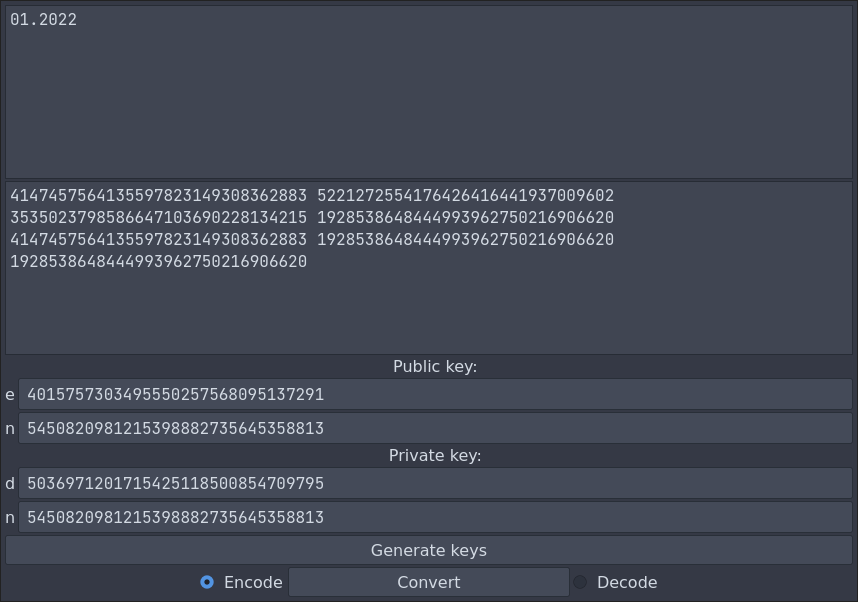
\includegraphics[width=0.8\linewidth]{figures/encode-test-3}}
    \caption{Шифрование}
\label{ris:encode-test-3}
\end{figure}

\vspace{\baselineskip}
\begin{figure}[H]
\center{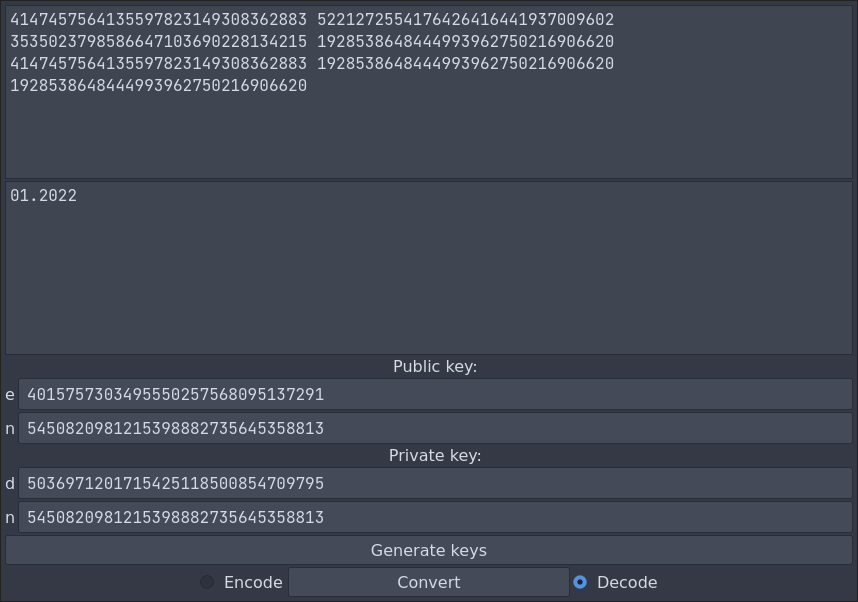
\includegraphics[width=0.8\linewidth]{figures/decode-test-3}}
    \caption{Расшифрование}
\label{ris:decode-test-3}
\end{figure}
